roughly 2-3 pages
\begin{itemize}
\item any details about experiments (dataset sizes, parameter selection, etc)
\item results
\item analysis (discussion of results/visualizations/findings/etc)
\end{itemize}

\subsection{Parameters}
For the experiments, the following parameters can be set:
\begin{itemize}
\item The $\alpha$ used for the extended LDA, which can be set from the command line using \verb|-a|. When not set, the default value of $0.1$ is used.
\item The $\beta$ used for the extended LDA, which can be set from the command line using \verb|-b|. When not set, the default value of $0.1$ is used.
\item The number of topics to be used, which can be set from the command line using \verb|-topics|. When not set, the default value of $50$ is used.
\item The number of iterations for Gibbs sampling, which can be set from the command line using \verb|-runs|. When not set, the default value of $1$ is used.
\end{itemize}

Each experiment has been run on the complete dataset of 9728 lyrics. A k-fold validation has been implemented to test the algorithm, which results in a non-biased test. 


It can be seen that the extension of LDA puts out more sensible topics than regular LDA: for example, after 20 iterations, the top words of the top topic of the reggae genre are \verb|yeah|, \verb|get|, \verb|got|, \verb|right|, \verb|man|, \verb|like|, \verb|little|, \verb|time|, \verb|say| and \verb|hey| using regular LDA, and \verb|mi|, \verb|fight|, \verb|police|, \verb|gonna|, \verb|say|, \verb|jah|, \verb|whatcha|, \verb|dem|, \verb|ya|, \verb|yuh|, \verb|burnin| and \verb|ah| using the extension of LDA. \textbf{VERMOEDEN, KAN PAS NA TESTS ECHT GEZEGD WORDEN} This results in a more effective classifier: \textbf{INSERT RESULTS.}

\begin{figure}
        \centering
        \begin{subfigure}[b]{0.3\textwidth}
                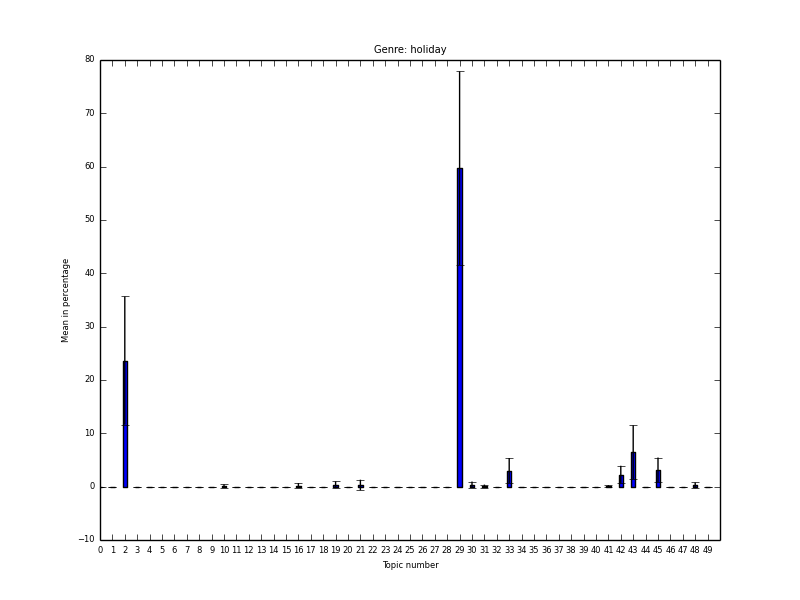
\includegraphics[width=\textwidth]{bar_charts/holiday.png}
                \caption{Genre Holiday}
                \label{fig:topicdist_holiday}
        \end{subfigure}%
        ~ %add desired spacing between images, e. g. ~, \quad, \qquad, \hfill etc.
          %(or a blank line to force the subfigure onto a new line)
        \begin{subfigure}[b]{0.3\textwidth}
                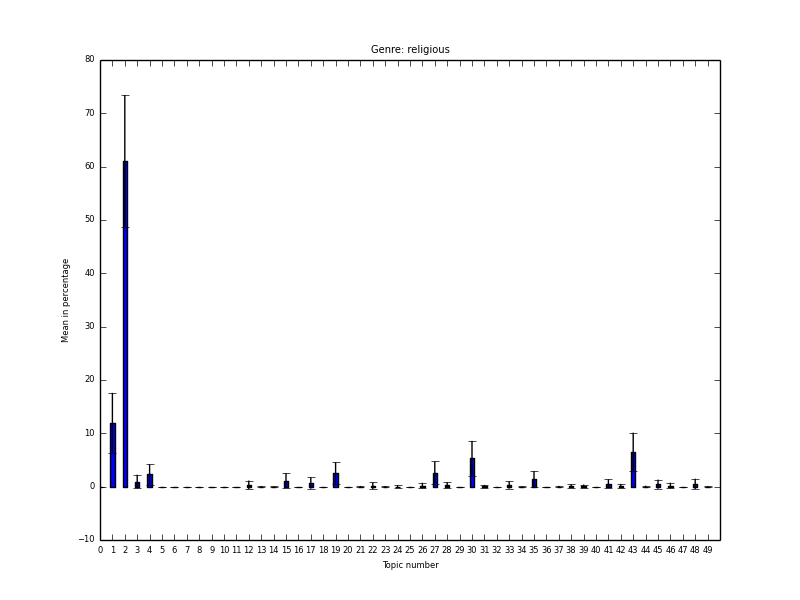
\includegraphics[width=\textwidth]{bar_charts/religious.png}
                \caption{Genre religious}
                \label{fig:topicdist_religious}
        \end{subfigure}
        ~ %add desired spacing between images, e. g. ~, \quad, \qquad, \hfill etc.
          %(or a blank line to force the subfigure onto a new line)
        \begin{subfigure}[b]{0.3\textwidth}
                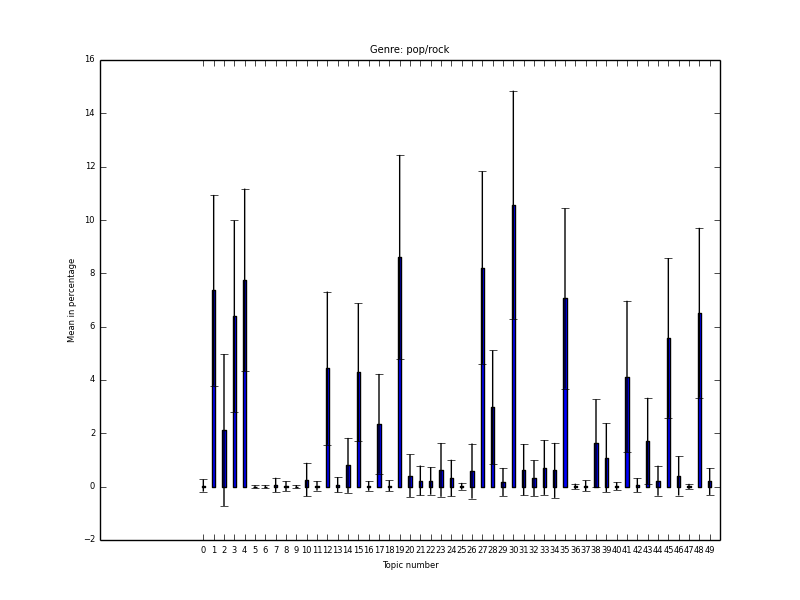
\includegraphics[width=\textwidth]{bar_charts/pop-rock.png}
                \caption{Genre pop/rock}
                \label{fig:topicdist_poprock}
        \end{subfigure}
        \begin{subfigure}[b]{0.3\textwidth}
                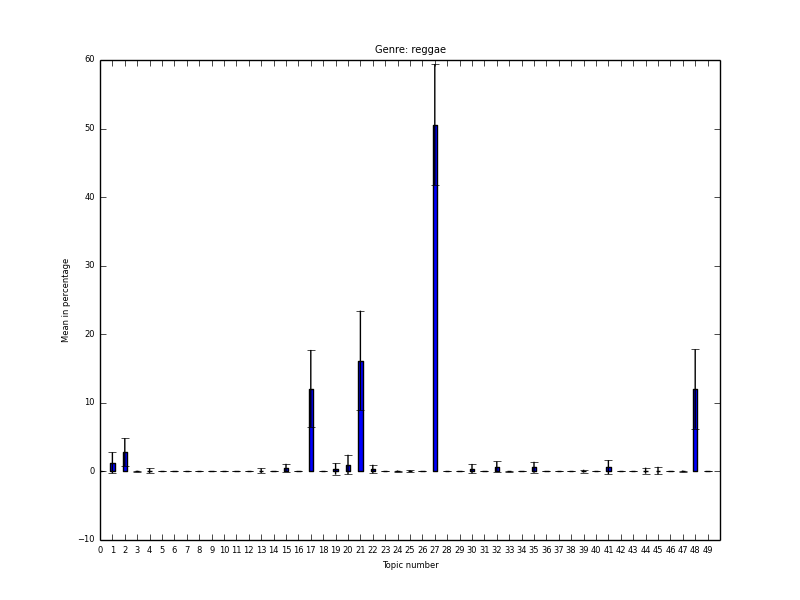
\includegraphics[width=\textwidth]{bar_charts/reggae.png}
                \caption{Genre Reggae}
                \label{fig:topicdist_reggae}
        \end{subfigure}%
        ~ %add desired spacing between images, e. g. ~, \quad, \qquad, \hfill etc.
          %(or a blank line to force the subfigure onto a new line)
        \begin{subfigure}[b]{0.3\textwidth}
                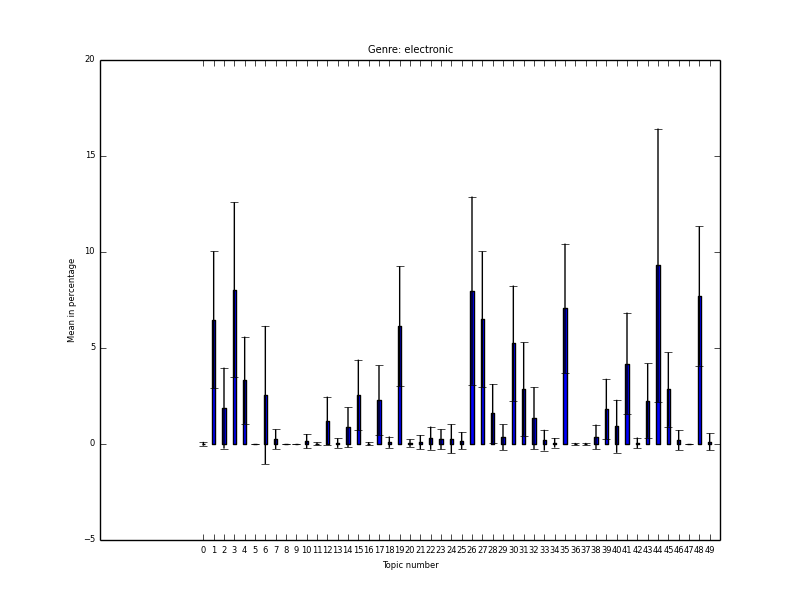
\includegraphics[width=\textwidth]{bar_charts/electronic.png}
                \caption{Genre Electronic}
                \label{fig:topicdist_electronic}
        \end{subfigure}
        ~ %add desired spacing between images, e. g. ~, \quad, \qquad, \hfill etc.
          %(or a blank line to force the subfigure onto a new line)
        \begin{subfigure}[b]{0.3\textwidth}
                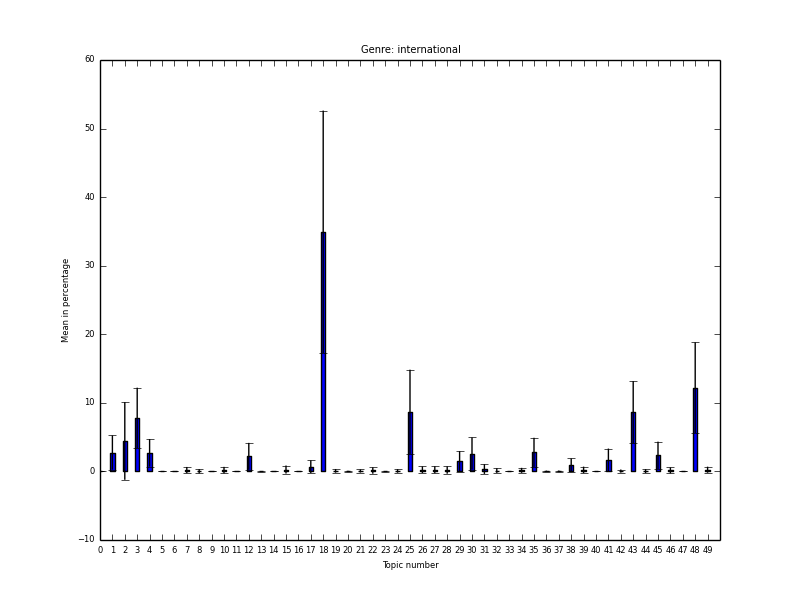
\includegraphics[width=\textwidth]{bar_charts/international.png}
                \caption{Genre International}
                \label{fig:topicdist_international}
        \end{subfigure}
        \caption{Topic distibution for different genres}\label{fig:topicdist}
\end{figure}